\documentclass[leqno,presentation,usenames,dvipsnames]{beamer}
\DeclareGraphicsExtensions{.eps,.jpg,.png,.tif}
\usepackage{amssymb, amsmath, pdfpages, amsfonts, calc, times, type1cm, latexsym, xcolor, colortbl, hyperref, bookmark}
\usepackage{graphicx}
\usepackage{tabularx}
\usepackage{multirow}
\usepackage{listings}
\graphicspath{ {images/} }

\usepackage[latin1]{inputenc}
\usepackage[english]{babel}

\usetheme{Szeged}
\usecolortheme{beaver}

\definecolor{websiteGreen}{RGB}{107, 224, 134}
\definecolor{silvery}{RGB}{232, 241, 248}
\definecolor{deepOrange}{RGB}{209, 126, 0}

\definecolor{softTan}{RGB}{240, 240, 223}
\definecolor{deepGreen}{RGB}{87, 149, 115}
\definecolor{lilac}{RGB}{199, 164, 202}
\definecolor{lightOlive}{RGB}{168, 166, 96}
\definecolor{deepOlive}{RGB}{101, 109, 41}

\setbeamercolor*{palette primary}{bg=websiteGreen}
\setbeamercolor*{palette secondary}{bg=white}
\setbeamercolor*{palette tertiary}{bg=silvery}
\setbeamercolor*{palette quaternary}{bg=websiteGreen}

\setbeamercolor{section in head/foot}{fg=black}
\setbeamerfont{section in head/foot}{series=\bfseries}

\setbeamercolor{titlelike}{parent=palette primary,bg=websiteGreen,fg=white}
\setbeamercolor{frametitle}{parent=palette primary,bg=websiteGreen, fg=white}

\addtobeamertemplate{frametitle}{\vspace*{-0.65\baselineskip}}{}


\newcommand{\R}{\mathbb{R}}
\newcommand{\N}{\mathbb{N}}
\newcommand{\overbar}[1]{\mkern1.5mu\overline{\mkern-1.5mu#1\mkern-1.5mu}\mkern1.5mu}
\newcommand{\highlight}[1]{
  \addtolength{\fboxrule}{.2ex}
  \begin{block}{}
    \begin{quote}#1
    \end{quote}
  \end{block}
}

\newtheorem*{conjecture}{Conjecture}
\newtheorem*{proposition}{Proposition}

\title{Automatic Theorem Proving}
\author[names]{%
    Reed Oei, Eric Ma \\ 
    Christian Schulz (Team Leader) \\ 
    Philipp Hieronymi (Faculty Mentor)
}

\institute{%
    University of Illinois at Urbana-Champaign, Illinois Geometry Lab 
}

\titlegraphic{%
  \includegraphics[width = 0.3\textwidth]{UIUC_logo.png}
  \hspace{.30cm}
  
\includegraphics[width = 0.07\textwidth]{igl-logo-small.png}
}

\date{May 2020}

\lstdefinelanguage{pecan}{
	keywords=[1]{forall, exists, max, min, sup, inf, are, is, if, then, match, with, case, end, let, be, in, else, iff},
	keywordstyle=[1]\color{blue}\bfseries,
	keywords=[2]{false, true, sometimes},
	commentstyle=\color{CadetBlue}\textit,
	stringstyle=\color{ForestGreen}, % string literal style
	keywordstyle=[2]\color{orange}\bfseries,
	keywords=[3]{assert_prop,Structure,defining,Theorem,Prove,Example,Alias,Restrict,Define,Display,Execute,load,shuffle,import,save_aut,save_aut_img,that,context,end_context,forget,shuffle,shuffle_or,using,of},
	keywordstyle=[3]\color{teal}\bfseries,
	keywords=[4]{@annotation,@postprocess,@no_simplify,@simplify,@simplify_states,@simplify_edges},
	keywordstyle=[4]\color{purple}\bfseries,
	literate=%
	    {\#}{{{\color{teal}\bfseries\#}}}1
	    {+}{{{\color{red}+~}}}1
	    {-}{{{\color{red}-~}}}1
        {:=}{{{\color{red}:=~}}}1
        {..}{{{\color{red}..~}}}1
        {\{}{{{\color{red}\{}}}1
        {\}}{{{\color{red}\}}}}1
        {|}{{{$\color{red} \lor~$}}}1
        {*}{{{\color{red}*~}}}1
        {:}{{{\color{red}:~}}}1
        {>}{{{\color{red}>~}}}1
        {<}{{{\color{red}<~}}}1
        {<=>}{{{$\color{red}\Leftrightarrow~$}}}1
        % <= conflicts with <=> as iff, so I commented it out because it's more importnat that <=> not look weird (it becomes \leq > with the following line).
        % But might as well keep something, so I keep \iff
        % {<=}{{{$\color{red} \leq$}}}1
        % Also got rid of >= for consistency.
        % {>=}{{{$\color{red} \geq$}}}1
        {.}{{{\color{red}.~}}}1
        {&}{{{$\color{red} \land~$}}}1
        {!}{{{$\color{red}\lnot~$}}}1
        {!=}{{{$\color{red} \neq$}}}1
        {=}{{{\color{red}=~}}}1
        {exists }{{{$\color{red}\exists$}}}1
        {forall }{{{$\color{red}\forall$}}}1,
    sensitive=false, % keywords are not case-sensitive
    morecomment=[l]{//}, % l is for line comment
    morecomment=[s]{/*}{*/}, % s is for start and end delimiter
    morestring=[b]", % defines that strings are enclosed in double quotes
    showstringspaces=false
}

\lstnewenvironment{pecan}
  {
    \lstset{
        language=pecan, 
        basicstyle=\small\ttfamily, 
        mathescape=true
        }
  }
  {
  }

\lstnewenvironment{pecan_output}
  {
    \lstset{
        basicstyle=\small\ttfamily,
        mathescape=true
        }
  }
  {
  }

\newcommand{\pecaninline}[1]{\lstinline[language=pecan,basicstyle=\small\ttfamily,mathescape]{#1}}


\begin{document}

% Title slide
\frame{\titlepage}

\section{Theorem Proving}

\begin{frame}{Automatic Theorem Proving}
    \begin{itemize}
        \item An \emph{automated theorem prover} is a program that takes a statement and proves (or disproves) it.
            \begin{itemize}
                \item Computers are reliable and fast
                \item We can easily explore new ideas
            \end{itemize}
            
        \item It is impossible to prove \textbf{all} statements automatically
        
        \item Theorem provers can still solve many interesting problems
    \end{itemize}
    
    \begin{figure}
        \centering
        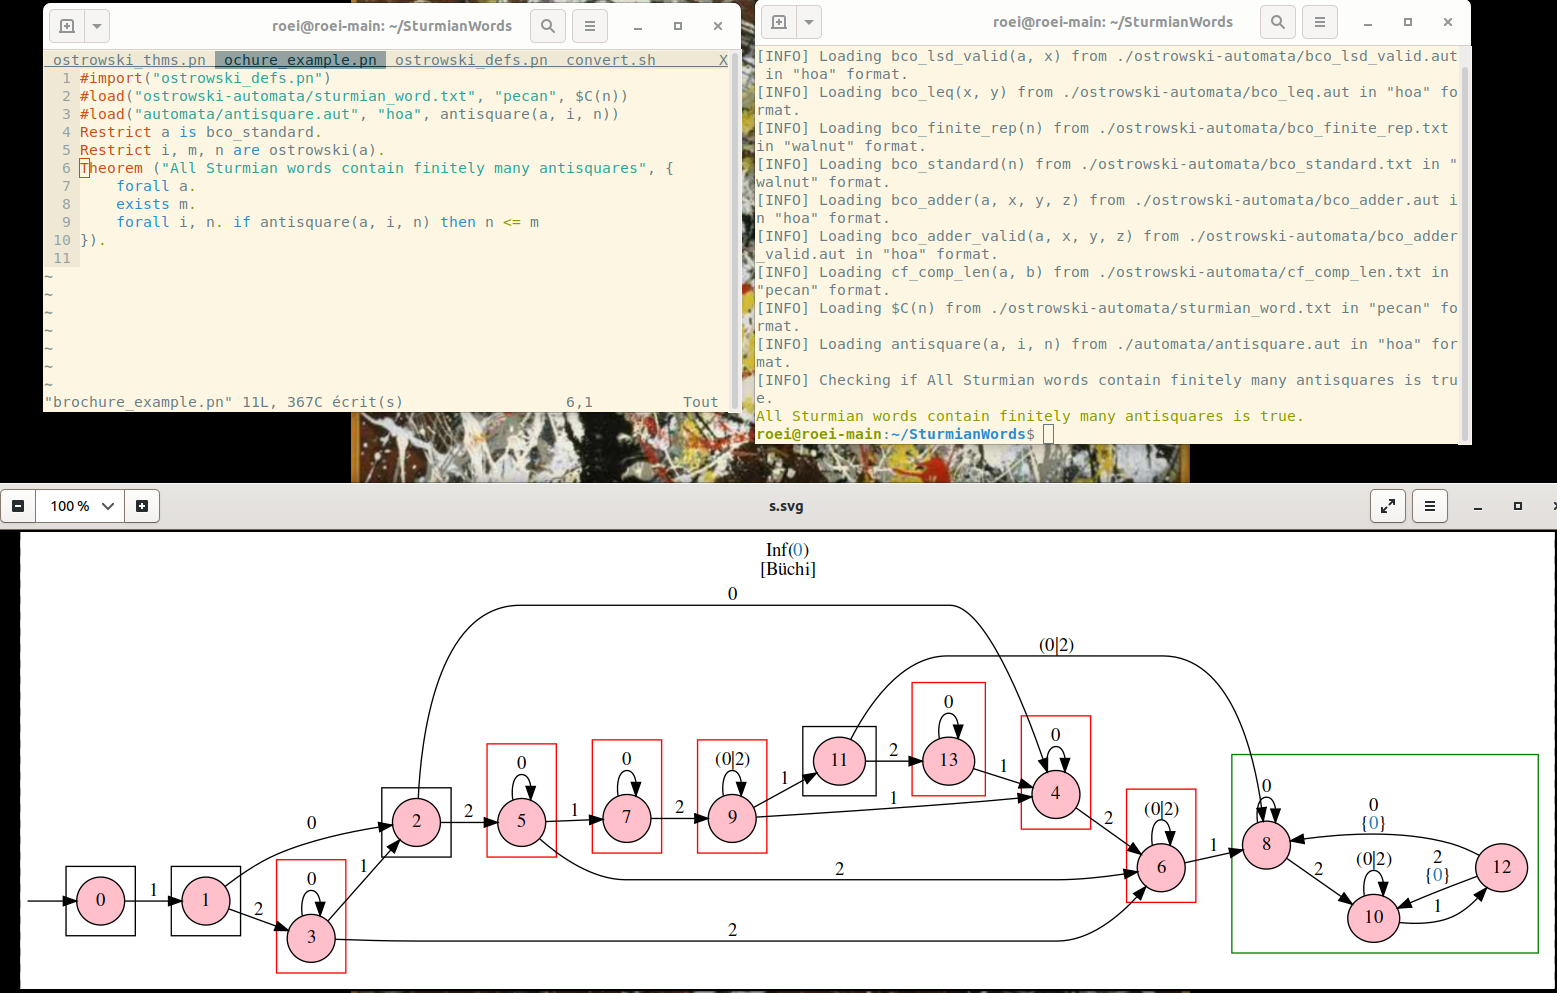
\includegraphics[width=0.5\textwidth]{images/pecan-demo-sp2020.png}
        \caption{A Pecan program and its output.}
        \label{fig:pecan-ex}
    \end{figure}
\end{frame}

\section{Pecan}
\begin{frame}[fragile]{Pecan}

\begin{itemize}
    \item \textbf{Pecan} is an automated theorem prover we are developing
    \item It represents logical statements via B\"uchi automata, a model of computation that can handle infinitely long inputs
    \item Try it online at \url{http://reedoei.com/pecan}!
\end{itemize}
    
\begin{pecan}
y is successor(x) := x < y & forallz. z <= x | y <= z
\end{pecan}

\begin{pecan}
Theorem ("Equality is symmetric.", { 
    forallx,y. x = y iff y = x 
}).
\end{pecan}
\end{frame}

\begin{frame}{Features of Pecan}
    \begin{itemize}
        \item A completely automatic theorem proving process for statements expressable with B\"uchi automata.
        \item Automata-based theorem proving is constructive: we can generate counterexamples of false statements.
        \item Support for custom numeration systems and \emph{automatic sequences} (sequences that can be calculated by an automaton)
    \end{itemize}
\end{frame}

\section{Examples}
\begin{frame}[fragile]{The Chicken McNugget Problem}
    
\begin{quote}
    What is the greatest number of chicken nuggets that cannot be ordered using only boxes of 6, 9, and 20?
\end{quote}

\begin{pecan}
n is purchasable := existsa,b,c. n =$\ $6*a $\color{red} +$ 9*b $\color{red} +$ 20*c
largest(n) := n = max { n : !(n is purchasable) }
\end{pecan}
\vspace{-1em}
\begin{figure}
    \centering
    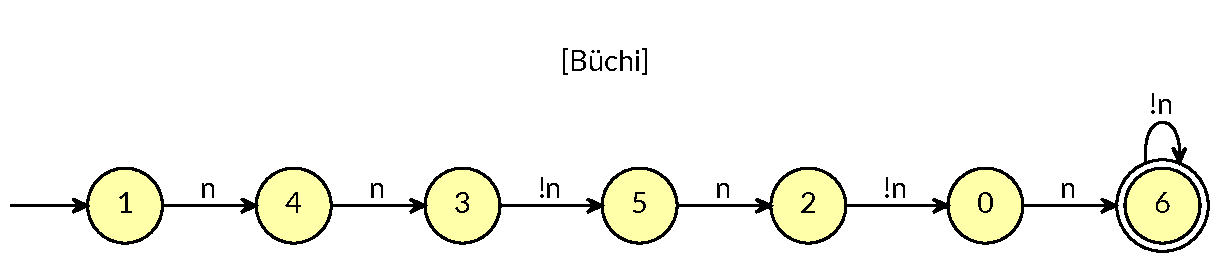
\includegraphics[width=\textwidth]{images/largest_not_purchasable.pdf}
    \caption{The B\"uchi automaton representing \pecaninline{largest(n)}, which accepts $110101_2$ ($43$ in base 10) in least significant digit first representation.}
    \label{fig:largest_non_purchasable}
\end{figure}
\end{frame}

\begin{frame}[fragile]{The Thue-Morse Word}
    \begin{itemize}
        \item $T[n] = 1$ if the binary representation of $n$ has an odd number of $1$'s, and $0$ otherwise.
        \[
            T = 01101001100101101001011001101001\ldots
        \]
        
        \item $p > 0$ is a \emph{period} of a word $w$ if $w$ repeats every $p$ letters; the smallest period of a word is its \emph{least period}.
        
    \end{itemize}
    
\begin{pecan}
p is period(i,j) := p > 0 &
    forallk. if i <= k & k < j-p then T[k]=T[k+p]
Prove that {
    forallp. if p > 0 then 
        existsi,j. p = min { m : period(i,j,m) }
}.
\end{pecan}
\end{frame}

\section{Sturmian Words}

\begin{frame}
    \frametitle{Sturmian Words}
    
    \begin{itemize}
        \item Imagine hitting a billiard ball at some angle along the line $y = \alpha x$
        \item When the ball crosses a vertical line, write a 0; for horizontal lines, write a 1
        \item Each $\alpha$ defines a \emph{characteristic Sturmian word}, $C_{\alpha}$
    \end{itemize}
    
\begin{figure}
    \centering
    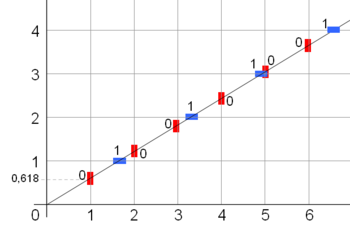
\includegraphics[width=0.5\textwidth]{images/Fibonacci_word_cutting_sequence.png}
    \caption{The characteristic Sturmian word $C_{1/\phi} = 0100101001\ldots$}
\end{figure}
\end{frame}

\begin{frame}{Theorems about Sturmian Words}
    We have used Pecan to automatically prove many theorems about Sturmian words, including:
    \begin{itemize}
        \item Sturmian words are not eventually periodic.
        \item All Sturmian words contain cubes.
        % \item Sturmian words start with arbitrarily long squares.
        \item Sturmian words contain palindromes of every length.
        \item Sturmian words contain only finitely many antisquares and antipalindromes.
        % \item If $x$ is a subword of a Sturmian word $C_{\alpha}$, then so is the reverse of $x$.
        \item Every subword of a Sturmian word occurs infinitely often.
        \item The unique special factor of length $n$ is the reverse of the length $n$ prefix of the Sturmian word.
        \item $\vdots$
    \end{itemize}
\end{frame}

\section{Future Work}
\begin{frame}{Future Work}
    \begin{enumerate}
        \item Continue to develop Pecan.
        \item Write a paper about Pecan and the various properties of Sturmian words we are able to automatically prove.
        \item Explore other applications of Pecan such as proving properties about real numbers or functions on real numbers, which are representable with B\"uchi automata but not finite automata.
    \end{enumerate}
\end{frame}

\end{document}
